\section{Introduction}

\begin{frame}
	\begin{block}{Product Quantization}
		In this report, we cover results of our experiments with the Product Quantization index (in particular, IVFPQ\footnotemark) \cite{Jegou2011} for the nearest neighbors search. The report includes the following:
		\begin{itemize}
			\item Showcase of IVFPQ performance on Oxford105K data (image descriptors with total number of samples $N = 104933$ of dimension $d = 128$);
			\item Comparison of IVFPQ with FLANN\footnotemark \cite{Muja2009}.
		\end{itemize}
	\end{block}
	
	\begin{block}{Technical Details}
		The implementation was performed using Python 3.7.7. The respective notebook is available on our \href{https://github.com/salisaresama/computer-vision/blob/master/product_quantization.ipynb}{{\color{blue}\underline{GitHub}}} page.
	\end{block}
	
	\addtocounter{footnote}{-2}
	\stepcounter{footnote}\footnotetext{We utilize Fair AI Similarity Search (\href{https://github.com/facebookresearch/faiss}{{\color{blue}\underline{faiss}}}) library with fixed parameters of the index: \texttt{nlist}$=100$, $m=16$, \texttt{nbits}$=8$, and \texttt{nprobe}$=32$ of IVFPQ index.}
	\stepcounter{footnote}\footnotetext{\href{https://github.com/primetang/pyflann}{{\color{blue} \underline{PyFLANN}}} library is used.}
\end{frame}


\section{Visual Assessment of IVFPQ Performance}
\subsection{Old Descriptors}

\begin{frame}
\frametitle{NN Search with IVFPQ on Old Image Descriptors}

\begin{figure}
\centering
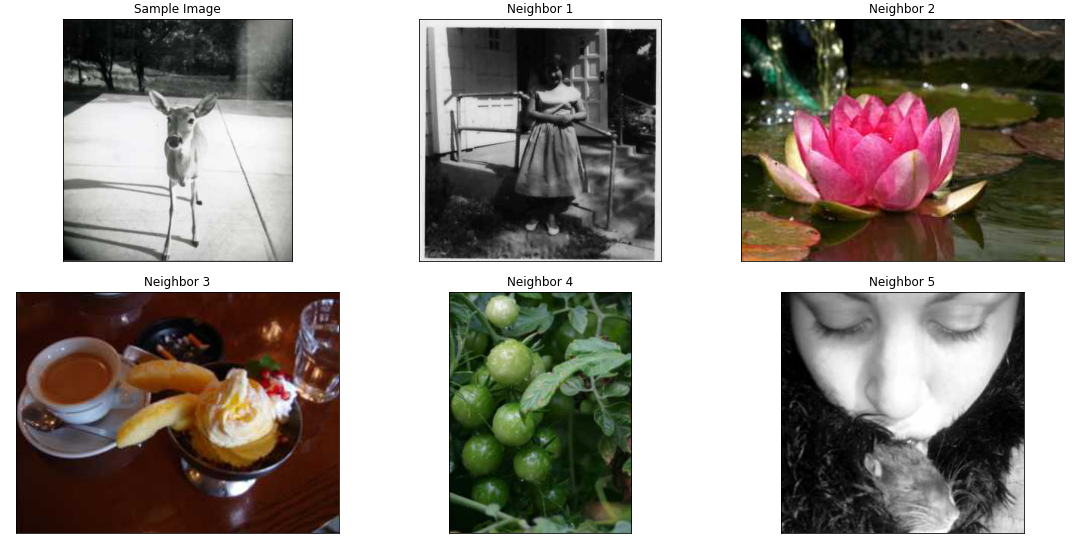
\includegraphics[width=0.85\linewidth]{../images/ivfpq/visual_assessment_old}
\caption{5 Nearest neighbors for the sample image. Not exhilarating performance on older image descriptors.}
\end{figure}

\end{frame}


\subsection{CNN-based Descriptors}

\begin{frame}
\frametitle{NN Search with IVFPQ on CNN-based Image Descriptors}

\begin{figure}
\centering
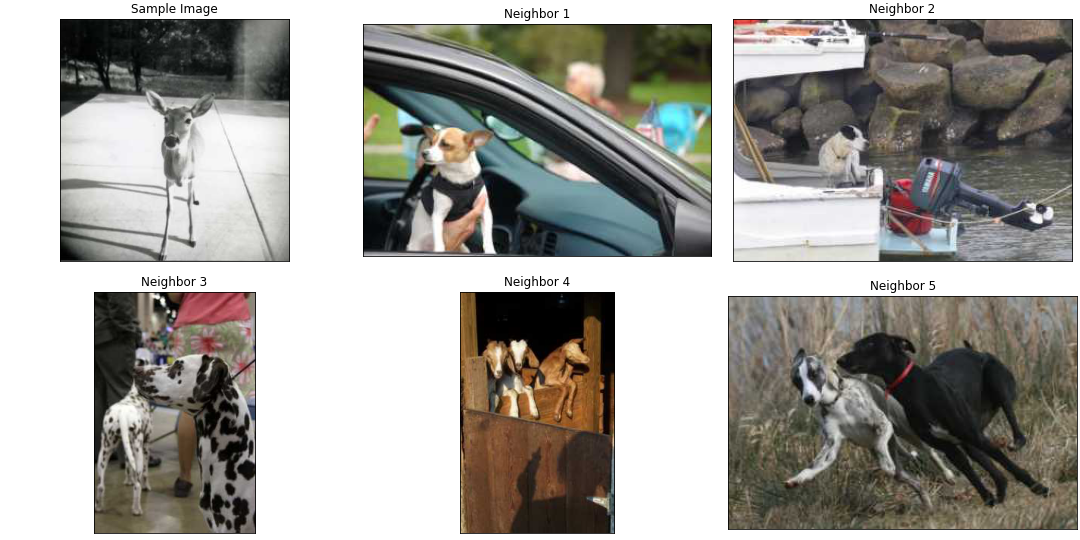
\includegraphics[width=0.85\linewidth,height=0.5\textheight]{../images/ivfpq/visual_assessment}
\caption{5 Nearest neighbors for the sample image. Better performance on CNN-based image descriptors, as all images at least depict animals with common features.}
\end{figure}

\end{frame}


\section{Quality of NN Search}
\subsection{Description and Timings}

\begin{frame}
	\begin{block}{Framework of the Experiment}
	\begin{itemize}
		\item We compare performance of IVFPQ with the k-d-forest (FLANN-KDF), the priority search k-means tree (FLANN-KMT), and the auto-tuned FLANN with target precision set to $0.99$ (FLANN-TARGET) by means of estimation of recall $R(k, K)$.\footnotemark
		\item Recall is measured as the average fraction over $1000$ queries (randomly selected images) of first $k$ true nearest neighbors found during the search of $K$ approximate nearest neighbors, $k \leq K$. Results for $K = 100$ can be viewed in Fig.~\ref{fig:comparison}.
		\item For each approach, we also measure the time to build the index and to perform the query. Results are presented in Tab.~\ref{tab:timings}.
	\end{itemize}

	\end{block}

\footnotesize{
\begin{table}
\centering
	\begin{tabular}{||c | c c ||} 
		\hline
		Method & Time to build the index, [s] & Time to perform the query, [s] \\ [0.5ex] 
		\hline\hline
		IVFPQ\footnotemark & 5.64 + 0.584 & 0.104  \\ 
		\hline
		FLANN-KDF & 4.24 & 0.1  \\
		\hline
		FLANN-KMT & 28.4 & 0.0582  \\
		\hline
		FLANN-TARGET & 28.2 & 0.0544  \\
		\hline
		Exact NN & - & 26  \\
		\hline
	\end{tabular}
	\caption{Timings of ANN methods to perform $1000$ queries for $100$ nearest neighbors.}
	\label{tab:timings}
\end{table}
}

\addtocounter{footnote}{-2}
 \stepcounter{footnote}\footnotetext{\scriptsize{FLANN parameters we used are available in the appendix (see Tab.~\ref{tab:flann-kdf-par} and Tab.~\ref{tab:flann-kmt-par}).}}
 \stepcounter{footnote}\footnotetext{Timings for both training on all data points and the point insertion are given.}
\end{frame}


\subsection{Recall}

\begin{frame}

\begin{figure}
\centering
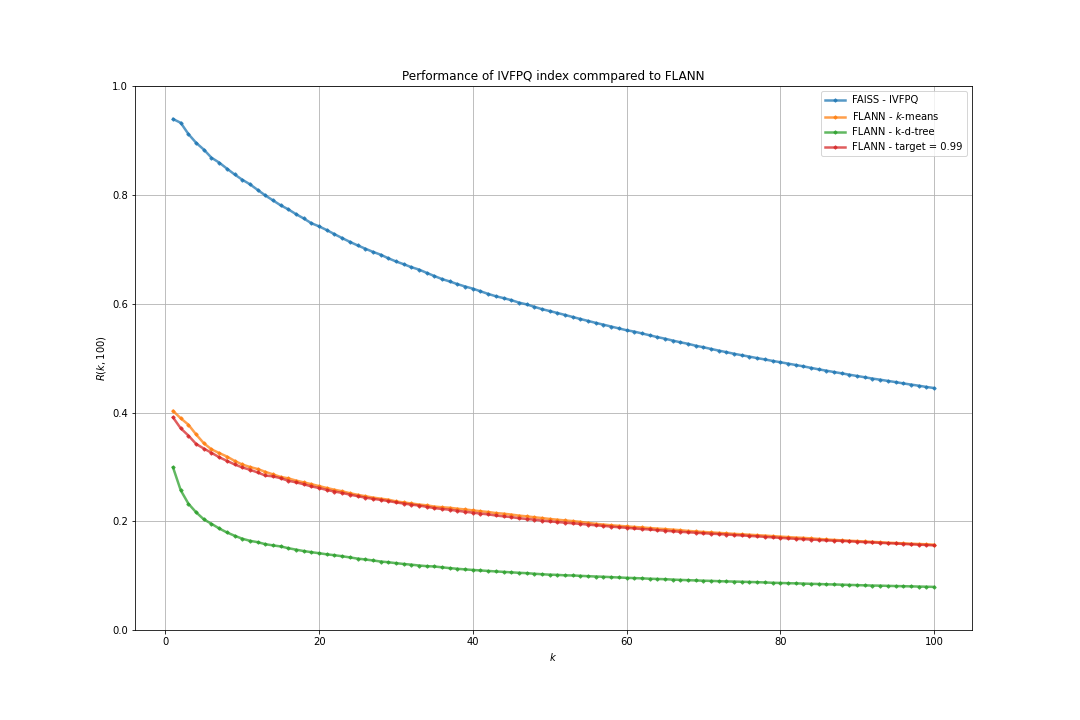
\includegraphics[width=0.9\linewidth]{../images/ivfpq/comparison}
\caption{Values of $R(k, 100)$. In terms of recall, IVFPQ demonstrates superior performance to FLANN.}
\label{fig:comparison}
\end{figure}

\end{frame}